%!TEX root = ../rapport.tex

\chapter{Contexte}

Comme dit précédemment, WinGo offre un service de TV sur Ip (IPTV). Il s'agit d'une Set-Top Box (STB) tournant sous Android qui reçoit le flux de données. Il est actuellement possible de mesurer la Qualité de Service (QoS) entre la plateforme de streaming IPTV et le routeur ADSL du client. Il n'est par contre pas possible de mesurer cette qualité entre le routeur et la STB. Le problème étant les différentes possibilités de connexions entre ces deux éléments, que cela soit par Ethernet ou par Wifi. Le but du projet est donc le développement d'une solution client (STB) - serveur (WinGo) permettant de mesurer la QoS.

\begin{figure}[H]
    \begin{center}
        \centering 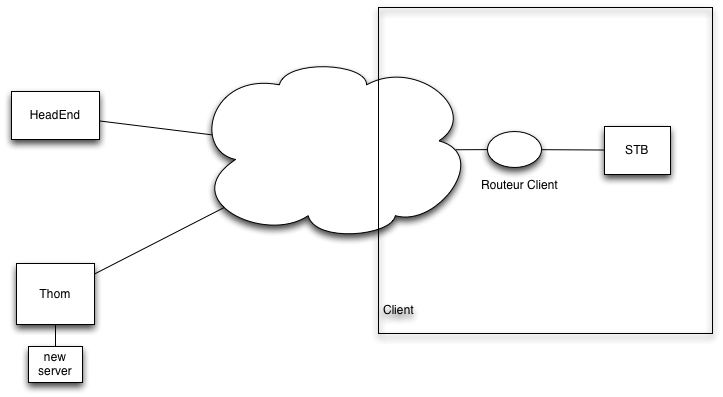
\includegraphics[width=0.7\linewidth]{CDC/schema_comm.png}
        \caption{Schéma de production actuel}
    \end{center}
\end{figure}

Voici l'environnement actuel en production, avec l'ajout d'un nouveau serveur.
\begin{itemize}
	\item Head End: C'est ici que les chaînes de TV sont reçues, encodées, encryptées et envoyées
	\item Thom: service de supervision. C'est ici que sont reportés tous les problèmes reportés avec leurs étapes de résolution.
	\item Serveur: C'est ici que l'implémentation côté serveur sera déployée
	\item Partie cliente: Routeur du client, connexion avec la STB qui contient le code Android permettant la communication avec notre nouveau serveur.
\end{itemize}

\medskip

La STB utilisée par WinGo est une box tournant sous Android. Il s'agit d'une surcouche graphique se superposant à l'image de la TV, donnant des informations supplémentaires comme la durée restante du programme en cours, le programme par chaînes etc. Il n'est pour le moment pas sûr que la box soit modifiable comme on le souhaite. C'est pourquoi dans un premier temps nous utiliserons un device tournant sous Android, à savoir une tablette Nexus 7 de Asus.
% section structure_du_document (end)